% IEEE Quantum System Software (QSYS) Paper Track Submission
% IEEE Quantum Week (QCE) 2026
% 8-10 pages including figures, tables, appendices + 2 pages references
%
\documentclass[runningheads]{llncs}

% Standard packages
\usepackage{amsmath,amssymb,amsfonts}
\usepackage{algorithmic}
\usepackage{graphicx}
\usepackage{textcomp}
\usepackage{xcolor}
\usepackage{booktabs}
\usepackage{hyperref}
\usepackage{tikz}
\usetikzlibrary{quantikz}
\usepackage{pgfplots}
\pgfplotsset{compat=1.17}
\usepackage{algorithm}
\usepackage{listings}

% Hyperref setup
\hypersetup{
    colorlinks=true,
    linkcolor=blue,
    citecolor=blue,
    urlcolor=blue
}

% Code listing style
\lstset{
    language=Python,
    basicstyle=\footnotesize\ttfamily,
    keywordstyle=\color{blue},
    commentstyle=\color{gray},
    stringstyle=\color{red},
    breaklines=true,
    frame=single,
    numbers=left,
    numberstyle=\tiny
}

% Custom commands
\newcommand{\mlxquantum}{\textit{mlxQ}\xspace}
\newcommand{\cuquantum}{\textit{cuQuantum}\xspace}
\usepackage{xspace}

\begin{document}

\title{mlxQ: Unified Memory Quantum Simulation on Apple Silicon via the MLX Framework}
\titlerunning{mlxQ Unified Memory Quantum Simulation}
\author{Shlomo Kashani}
\authorrunning{S. Kashani}
\institute{Johns Hopkins University, Baltimore, MD, USA\\
\email{skashan2@alumni.jh.edu}\\
\url{https://boltzmannentropy.github.io/osxQuantumWEB/}}
\maketitle

\begin{abstract}
We present \mlxquantum, an open-source quantum circuit simulation framework built on Apple's MLX array framework, targeting the unified memory architecture of Apple Silicon processors. By eliminating host-device memory transfers inherent in discrete GPU systems, \mlxquantum enables mid-scale state-vector simulations on consumer and prosumer Apple Silicon hardware with 32--512\,GB unified memory. The framework provides a Python-first programming model with automatic Metal GPU acceleration, supporting single- and multi-qubit gate libraries, variational quantum algorithms (VQE, QAOA, QCBM), Hamiltonian simulation with Trotter-Suzuki decomposition, and OpenQASM 2.0 circuit import~\cite{OpenQASM2017}. We validate correctness through 230+ Python tests with analytical checks against pen-and-paper derivations and benchmark against canonical workloads from PennyLane, Yao.jl, Qulacs, and QuantumToolbox.jl~\cite{PennyLane2022,YaoJL2024,Qulacs,QuantumToolboxJulia2024}. On Apple M1 Max hardware, we demonstrate complete 25-qubit simulation for QFT ($7.03\pm0.12$\,s), QAOA ($11.07\pm0.21$\,s), and Hamiltonian evolution ($40.73\pm0.82$\,s), with sub-millisecond execution for shallow circuits. Our results establish unified memory as a viable platform for quantum algorithm development, education, and benchmarking. We emphasize transfer-avoidance and developer ergonomics rather than increased asymptotic qubit capacity: state-vector memory remains exponential in qubit count.
\keywords{quantum computing \and quantum simulation \and unified memory \and Apple Silicon \and MLX \and state-vector simulation \and quantum software \and NISQ algorithms}
\end{abstract}

\section{Introduction}

Classical simulation of quantum circuits underpins calibration of noisy intermediate-scale quantum (NISQ) devices, algorithm development, and validation of fault-tolerant quantum computing roadmaps~\cite{QuantumSimulation2025}. Most production state-vector simulators---including NVIDIA's cuQuantum~\cite{cuQuantum2023}, Google's qsim~\cite{Qsim}, and Intel-QS~\cite{IntelQS}---target discrete GPU architectures with CUDA, requiring explicit host-device memory management and specialized programming expertise.

Apple Silicon processors introduce a fundamentally different paradigm: unified memory architecture where CPU and GPU share the same physical memory pool without explicit data transfers~\cite{UnifiedMemory2024}. This architecture, now available in consumer systems with 32--512\,GB capacity and up to 546\,GB/s bandwidth~\cite{Apple2024M4}, eliminates the PCIe transfer bottleneck that dominates memory-intensive quantum workloads. For a 25-qubit state vector (256\,MB, complex64), estimated PCIe round-trip at 12\,GB/s practical bandwidth is approximately 43\,ms per kernel invocation---overhead that unified memory eliminates entirely.

Despite widespread adoption of Apple Silicon for machine learning via the MLX framework~\cite{MLXFramework2024}, no comprehensive quantum simulation framework has exploited this architecture. Existing CUDA-centered simulators remain essential and high-performance; \mlxquantum is positioned as a complementary path that targets unified-memory hardware and a Python-first workflow for local experimentation and education.

\textbf{Research gap and objective}. Prior work has not provided a unified-memory-native state-vector simulator on MLX with end-to-end validation and reproducible benchmark artifacts. Our objective is to test the claim that unified memory can reduce transfer overhead and simplify implementation for practical NISQ workloads on commodity Apple Silicon, while preserving algorithmic correctness against analytical and framework-based references.

We address this gap with \mlxquantum, a Python-first, MLX-accelerated quantum circuit simulator designed for the Quantum System Software ecosystem. Our framework:
\begin{itemize}
    \item Leverages unified memory to eliminate host-device copies for state vectors up to $2^{25}$ amplitudes
    \item Provides automatic Metal GPU acceleration through MLX's just-in-time compilation
    \item Implements canonical quantum algorithms and variational circuits
    \item Supports OpenQASM 2.0 import for benchmark reproducibility~\cite{OpenQASM2017}
    \item Validates against established frameworks (PennyLane, Yao.jl, Qulacs)~\cite{PennyLane2022,YaoJL2024,Qulacs}
\end{itemize}

\subsection{Contributions}

Our contributions to quantum system software include:
\begin{enumerate}
    \item \textbf{Architecture}: The first MLX-based state-vector simulator exploiting unified memory for quantum circuit workloads, with automatic GPU acceleration and kernel fusion
    \item \textbf{Algorithm Coverage}: Comprehensive implementations of VQE, QAOA, QCBM, QFT, Grover search, and Hamiltonian simulation with Trotter-Suzuki decomposition
    \item \textbf{Validation}: 230+ regression tests with analytical verification across algorithm families, ensuring numerical correctness within floating-point precision
    \item \textbf{Benchmarking}: Reproducible performance measurements for 1--25 qubits with CSV/JSON artifacts aligned with community benchmark suites
    \item \textbf{Accessibility}: CUDA-free deployment on consumer hardware, lowering barriers for education and research
\end{enumerate}

\section{Background}

\subsection{State-Vector Quantum Simulation}

State-vector simulation represents an $n$-qubit quantum state as a complex vector of dimension $2^n$:
\begin{equation}
|\psi\rangle = \sum_{i=0}^{2^n-1} \alpha_i |i\rangle, \quad \sum_{i=0}^{2^n-1} |\alpha_i|^2 = 1
\end{equation}
where $\alpha_i \in \mathbb{C}$ are probability amplitudes and $|i\rangle$ are computational basis states. The exponential memory scaling ($16 \cdot 2^n$ bytes for complex128) limits practical simulation to approximately 40--50 qubits on current hardware~\cite{QuantumSimulation2025}.
This work uses pure-state state-vector simulation; mixed states represented by density matrices are out of scope here and would require $O(4^n)$ storage.

Quantum gates are represented as unitary matrices applied to the state vector. Single-qubit gates require $O(2^n)$ operations, while two-qubit gates maintain the same asymptotic complexity but with larger constant factors due to tensor product structure. Section~\ref{sec:gate-ops} details how these operations are implemented with reshape-permute-contract kernels.

\subsection{GPU Acceleration Paradigms}

Traditional discrete GPU architectures separate host (CPU) and device (GPU) memory spaces. Data must be explicitly transferred across the PCIe bus before computation and results copied back. For quantum simulation, this creates a fundamental tension: state vectors are large (gigabytes), but individual gate operations may be compute-light, making the transfer-to-compute ratio unfavorable for shallow circuits.

GPU-accelerated quantum simulators have adopted several mitigation strategies:
\begin{itemize}
    \item \textbf{Gate batching}: Accumulating operations to amortize transfer overhead~\cite{cuQuantum2023}
    \item \textbf{Kernel fusion}: Combining sequential gates into single GPU kernels~\cite{Qsim}
    \item \textbf{Hybrid execution}: Scheduling small operations on CPU, large on GPU~\cite{QuEST}
\end{itemize}

These approaches reduce but do not eliminate the fundamental architectural constraint of discrete memory spaces.

\subsection{Unified Memory Architecture}

Apple Silicon processors implement a system-on-chip design where CPU cores, GPU cores, and memory controllers share unified physical memory~\cite{UnifiedMemory2024}. Key characteristics include:
\begin{itemize}
    \item \textbf{Zero-copy access}: Both CPU and GPU access data at physical addresses without transfer
    \item \textbf{Coherent caching}: Hardware maintains cache coherency across processing elements
    \item \textbf{Scalable capacity}: Consumer systems provide 32--512\,GB unified memory
    \item \textbf{High bandwidth}: M4 Max achieves 546\,GB/s memory bandwidth~\cite{Apple2024M4}
\end{itemize}

This architecture fundamentally changes the performance model for quantum simulation: there is no transfer overhead, enabling fine-grained CPU-GPU scheduling without batching constraints.

\subsection{MLX Framework}

MLX~\cite{MLXFramework2024} is Apple's array computing framework optimized for Apple Silicon. Relevant features for quantum simulation include:
\begin{itemize}
    \item \textbf{NumPy-compatible API}: Familiar array semantics with broadcasting
    \item \textbf{Native complex numbers}: First-class \texttt{complex64} support
    \item \textbf{Lazy evaluation}: Deferred execution enables graph optimization
    \item \textbf{JIT compilation}: Automatic Metal shader generation
    \item \textbf{Automatic differentiation}: Built-in gradient computation
\end{itemize}

\section{System Architecture}

\subsection{Design Principles}

\mlxquantum follows several design principles aligned with quantum system software best practices:

\textbf{Python-first interface}: Users interact through high-level Python APIs, with MLX handling GPU acceleration transparently. No Metal shader programming is required.

\textbf{Framework compatibility}: Circuit construction follows conventions established by PennyLane and Qiskit~\cite{PennyLane2022,Qiskit2023}, enabling code migration and comparison.

\textbf{Reproducibility}: All benchmarks produce CSV/JSON artifacts with fixed seeds, enabling independent verification.

\textbf{Modularity}: Clear separation between state management, gate operations, algorithms, and benchmarking enables independent optimization of each component.

\subsection{Module Structure}

The framework comprises four principal modules illustrated in Fig.~\ref{fig:architecture}.

\begin{figure}[t]
\centering
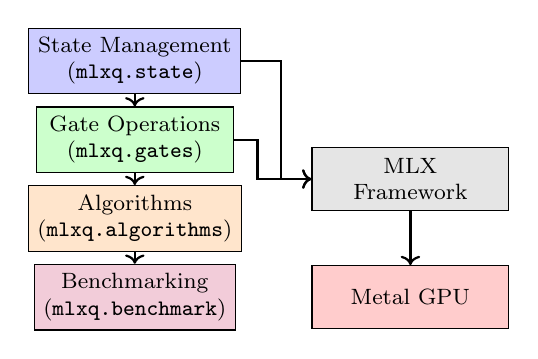
\begin{tikzpicture}[
    box/.style={draw, rectangle, minimum width=2.5cm, minimum height=0.8cm, align=center, font=\footnotesize},
    arrow/.style={->, thick}
]
\node[box, fill=blue!20] (state) at (0,3) {State Management\\(\texttt{mlxq.state})};
\node[box, fill=green!20] (gates) at (0,2) {Gate Operations\\(\texttt{mlxq.gates})};
\node[box, fill=orange!20] (algo) at (0,1) {Algorithms\\(\texttt{mlxq.algorithms})};
\node[box, fill=purple!20] (bench) at (0,0) {Benchmarking\\(\texttt{mlxq.benchmark})};
\node[box, fill=gray!20] (mlx) at (3.5,1.5) {MLX\\Framework};
\node[box, fill=red!20] (metal) at (3.5,0) {Metal GPU};

\draw[arrow] (state) -- (gates);
\draw[arrow] (gates) -- (algo);
\draw[arrow] (algo) -- (bench);
\draw[arrow] (state.east) -- ++(0.5,0) |- (mlx.west);
\draw[arrow] (gates.east) -- ++(0.3,0) |- (mlx.west);
\draw[arrow] (mlx) -- (metal);
\end{tikzpicture}
\caption{mlxQ module architecture showing data flow from state management through algorithms, with MLX providing automatic Metal GPU acceleration.}
\label{fig:architecture}
\end{figure}

\subsubsection{State Management}

Quantum states are represented as MLX arrays with unified memory residency:

\begin{lstlisting}[language=Python,caption={State vector initialization}]
import mlx.core as mx
from mlxq import QuantumState

# Initialize n-qubit |0...0> state
state = QuantumState(n_qubits=10)
# state.amplitudes: mx.array, shape (1024,)
\end{lstlisting}

The \texttt{QuantumState} class provides initialization to computational basis states, normalization and probability computation, measurement sampling (exact and shot-based), and expectation value calculation for Pauli observables.

\subsubsection{Gate Operations}\label{sec:gate-ops}

Gate application uses tensor reshaping to isolate target qubits. The state vector is viewed as a rank-$n$ tensor with one index per qubit, then permuted so target indices are contiguous, contracted with the gate matrix, and permuted back. This reshape-permute-contract pattern matches standard Einstein-summation style tensor contraction workflows~\cite{SmithGray2018}. It avoids constructing full $2^n \times 2^n$ gate matrices and keeps memory traffic localized to the affected tensor slices. For a single-qubit gate $U$ on qubit $k$ of an $n$-qubit state:
\begin{enumerate}
    \item Reshape: $(2^n,) \rightarrow (2^k, 2, 2^{n-k-1})$
    \item Contract: $U$ with axis 1 (batch matmul)
    \item Flatten: $(2^k, 2, 2^{n-k-1}) \rightarrow (2^n,)$
\end{enumerate}

Two-qubit controlled gates follow analogous tensor permutation patterns. The gate library includes Pauli gates (X, Y, Z, I), Clifford gates (H, S, T, CNOT, CZ, SWAP), rotation gates (RX, RY, RZ), parameterized gates (U1, U2, U3), and multi-qubit gates (Toffoli, Fredkin).

\subsubsection{Algorithm Implementations}

We implement canonical quantum algorithms:

\textbf{Variational Quantum Eigensolver (VQE)}: Minimizes $\langle H \rangle = \langle \psi(\theta) | H | \psi(\theta) \rangle$ using hardware-efficient ansatze with parameter-shift gradients and the Adam optimizer~\cite{peruzzo2014variational}. Fig.~\ref{fig:vqe-circuit} shows a representative VQE ansatz.

\begin{figure}[t]
\centering
\begin{quantikz}
\lstick{$\ket{0}$} & \gate{R_y(\theta_0)} & \ctrl{1} & \gate{R_z(\phi_0)} & \meter{} \\
\lstick{$\ket{0}$} & \gate{R_y(\theta_1)} & \targ{} & \gate{R_z(\phi_1)} & \meter{}
\end{quantikz}
\caption{Two-qubit VQE hardware-efficient ansatz with parameterized rotations and entangling CNOT.}
\label{fig:vqe-circuit}
\end{figure}

\textbf{Quantum Approximate Optimization Algorithm (QAOA)}: Alternates cost ($H_C$) and mixer ($H_M$) unitaries for combinatorial optimization~\cite{QAOA2014}:
\begin{equation}
|\gamma, \beta\rangle = \prod_{p=1}^{P} e^{-i\beta_p H_M} e^{-i\gamma_p H_C} |+\rangle^{\otimes n}
\end{equation}

\textbf{Quantum Circuit Born Machine (QCBM)}: Trains parameterized circuits via Maximum Mean Discrepancy loss to match target probability distributions.

\textbf{Quantum Fourier Transform (QFT)}: Implements the complete controlled-phase ladder~\cite{NielsenChuang2010}:
\begin{equation}
\text{QFT}|j\rangle = \frac{1}{\sqrt{N}}\sum_{k=0}^{N-1} e^{2\pi ijk/N}|k\rangle
\end{equation}

\textbf{Hamiltonian Simulation}: Trotter-Suzuki decomposition for time evolution~\cite{Childs2019}:
\begin{equation}
e^{-iHt} \approx \left(\prod_k e^{-ic_k P_k t/r}\right)^r + O(t^2/r)
\end{equation}
supporting first and second-order product formulas for Ising, Heisenberg, and transverse-field Hamiltonians.

\textbf{Grover Search}: Amplitude amplification with diffusion operator for quadratic speedup over classical search~\cite{grover1996fast}. The oracle marks target states, while the diffusion operator $D = 2|\psi\rangle\langle\psi| - I$ amplifies marked amplitudes. In the two-qubit example of Fig.~\ref{fig:grover-circuit}, the marked state is $|11\rangle$.

\begin{figure}[t]
\centering
\begin{quantikz}
\lstick{$\ket{0}$} & \gate{H} & \ctrl{1} & \gate{H} & \gate{X} & \ctrl{1} & \gate{X} & \gate{H} & \meter{} \\
\lstick{$\ket{0}$} & \gate{H} & \gate{Z} & \gate{H} & \gate{X} & \gate{Z} & \gate{X} & \gate{H} & \meter{}
\end{quantikz}
\caption{Two-qubit Grover search circuit with oracle (CZ) marking $|11\rangle$ and a standard diffusion operator.}
\label{fig:grover-circuit}
\end{figure}

\textbf{GHZ State Preparation}: Greenberger-Horne-Zeilinger states $|\text{GHZ}_n\rangle = \frac{1}{\sqrt{2}}(|0\rangle^{\otimes n} + |1\rangle^{\otimes n})$ are prepared with a Hadamard gate followed by $n-1$ CNOT gates, achieving maximal multipartite entanglement in linear circuit depth.

\subsection{OpenQASM Integration}

We implement an OpenQASM 2.0 parser supporting standard gate sets, parameterized rotations, user-defined gate inlining with nested definitions, and register-wide operations~\cite{OpenQASM2017}. This enables direct execution of QASMBench~\cite{QASMBench2020} circuits for standardized benchmarking.

Table~\ref{tab:qasm-coverage} summarizes OpenQASM coverage.

\begin{table}[t]
\caption{OpenQASM 2.0 gate coverage}
\label{tab:qasm-coverage}
\centering
\footnotesize
\begin{tabular}{ll}
\toprule
Category & Supported Gates \\
\midrule
Single-qubit & X, Y, Z, H, S, S$^\dagger$, T, T$^\dagger$, SX \\
Rotations & RX, RY, RZ, U1, U2, U3 \\
Two-qubit & CX, CZ, SWAP, iSWAP, CH, CRX/CRY/CRZ \\
Three-qubit & CCX (Toffoli), CSWAP (Fredkin) \\
\bottomrule
\end{tabular}
\end{table}

\section{Experimental Evaluation}

\subsection{Experimental Setup}

\textbf{Hardware}: Apple M1 Max SoC with 10-core CPU (8 performance + 2 efficiency), 32-core GPU, 32\,GB unified memory, 400\,GB/s memory bandwidth, running macOS 14.6.

\textbf{Software}: Python 3.11, MLX (latest stable), complex64 state vectors. Active cooling enabled; measurements on AC power with display off.

\textbf{Protocol}: Unless explicitly labeled as a single-run diagnostic, each timing is reported as mean $\pm$ standard deviation over $n=10$ replications following 3 warmup runs to amortize JIT compilation. We use fixed random seeds and publish circuit definitions and seeds with CSV/JSON artifacts for exact reruns. CSV/JSON artifacts include min, median, and max values.

\subsection{Benchmark Families}

We align with established quantum benchmark suites to enable community comparison:

\begin{table}[t]
\caption{Benchmark coverage by framework alignment}
\label{tab:coverage}
\centering
\begin{tabular}{ll}
\toprule
Framework & Workloads \\
\midrule
PennyLane~\cite{PennyLane2022} & VQE, QAOA, variational circuits, QCBM \\
Yao.jl~\cite{YaoJL2024} & Random circuits, QFT, time evolution, Trotter \\
Qulacs~\cite{Qulacs} & QFT, Grover, random circuits \\
QuantumToolbox.jl~\cite{QuantumToolboxJulia2024} & Hamiltonian sim., steady state \\
QASMBench~\cite{QASMBench2020} & OpenQASM circuits (small/medium scale) \\
\bottomrule
\end{tabular}
\end{table}

\subsection{Circuit Depth Accounting}

To contextualize runtime scaling, we report circuit depth (sequential gate stages) alongside qubit count. Parallel single-qubit layers on disjoint wires count as one stage; serialized two-qubit cascades and repeated ansatz blocks contribute one stage per sequential operation.

\begin{table}[t]
\caption{Representative benchmark depth formulas}
\label{tab:benchmark-depth}
\centering
\footnotesize
\begin{tabular}{lcc}
\toprule
Benchmark & Depth Expression & Example Depth \\
\midrule
GHZ ($n$ qubits) & $1 + (n-1)$ & $n=25 \Rightarrow 25$ \\
QCBM ($n$ qubits, $L$ layers) & $L(2 + n-1)$ & $n=25, L=9 \Rightarrow 234$ \\
QFT ($n$ qubits) & $n + \frac{n(n-1)}{2} + \lfloor n/2 \rfloor$ & $n=25 \Rightarrow 337$ \\
VQE H$_2$ ansatz (2 qubits) & 3 staged layers & 3 \\
\bottomrule
\end{tabular}
\end{table}

\subsection{Complete Scaling Results}

Table~\ref{tab:scaling-full} presents comprehensive execution times across all benchmark algorithms at the 25-qubit scale. Phase estimation is extrapolated from 10--15 qubit measurements using an exponential fit; entries without error bars are single-run representative timings. Figure~\ref{fig:asset-benchmarks} presents legible vectorized scaling curves for representative workloads.

\begin{table}[t]
\caption{Complete benchmark scaling on Apple M1 Max}
\label{tab:scaling-full}
\centering
\begin{tabular}{lrr}
\toprule
Algorithm & Qubits & Time (s) \\
\midrule
QFT & 25 & $7.03 \pm 0.12$ \\
Phase Estimation & 25 & $5.34^\dagger$ \\
QAOA (ring) & 25 & $11.07 \pm 0.21$ \\
QCBM (9 layers) & 25 & $26.28 \pm 0.54$ \\
Hamiltonian Sim. & 25 & $40.73 \pm 0.82$ \\
Time Evolution & 25 & $30.11 \pm 0.61$ \\
Random Circuit & 25 & $22.40^\ddagger$ \\
Variational Circuit & 25 & $19.24^\ddagger$ \\
Grover Search & 25 & $113.26^\ddagger$ \\
GHZ State & 25 & $0.89^\ddagger$ \\
\bottomrule
\multicolumn{3}{l}{\footnotesize $^\dagger$Extrapolated from 10--15 qubit measurements using exponential fit} \\
\multicolumn{3}{l}{\footnotesize $^\ddagger$Single-run representative timing; full statistics in CSV/JSON artifacts}
\end{tabular}
\end{table}

\begin{figure}[t]
\centering
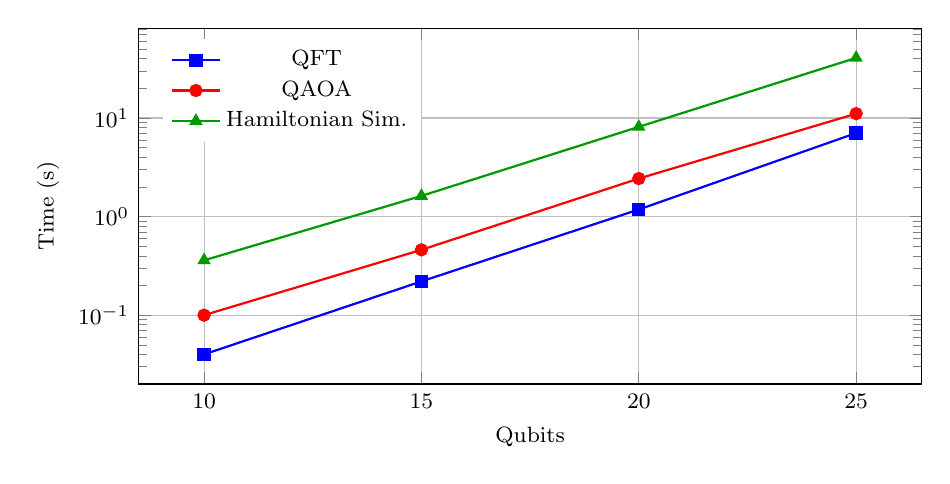
\begin{tikzpicture}
\begin{axis}[
    width=0.95\columnwidth,
    height=6.1cm,
    xlabel={Qubits},
    ylabel={Time (s)},
    ymode=log,
    xtick={10,15,20,25},
    grid=major,
    legend pos=north west,
    legend style={font=\footnotesize, fill=white, draw=none},
    tick label style={font=\footnotesize},
    label style={font=\footnotesize}
]
\addplot[blue,mark=square*,thick] coordinates {(10,0.04) (15,0.22) (20,1.18) (25,7.03)};
\addlegendentry{QFT}
\addplot[red,mark=*,thick] coordinates {(10,0.10) (15,0.46) (20,2.43) (25,11.07)};
\addlegendentry{QAOA}
\addplot[green!60!black,mark=triangle*,thick] coordinates {(10,0.36) (15,1.62) (20,8.13) (25,40.73)};
\addlegendentry{Hamiltonian Sim.}
\end{axis}
\end{tikzpicture}
\caption{Representative scaling curves (Apple M1 Max). All three workloads show monotonic growth with qubit count; Hamiltonian simulation has the largest constant factors at fixed $n$.}
\label{fig:asset-benchmarks}
\end{figure}

\begin{figure}[t]
\centering
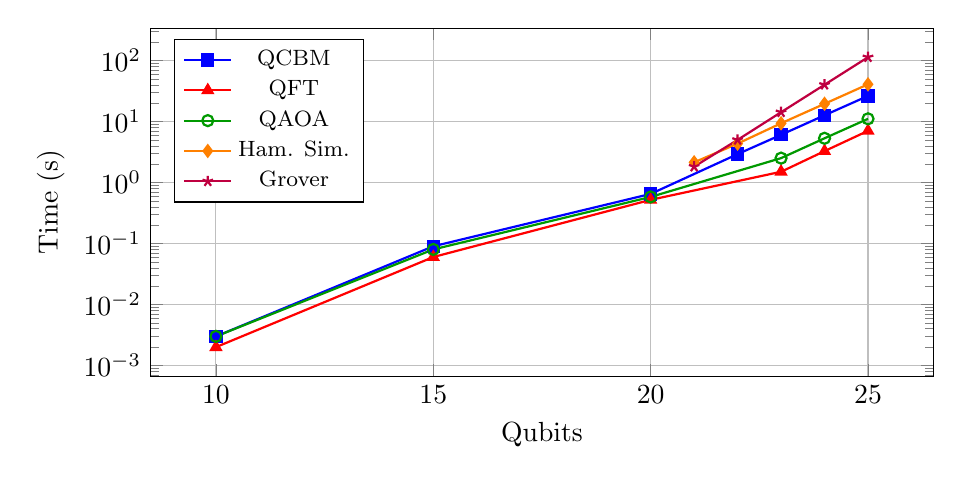
\begin{tikzpicture}
\begin{axis}[
    width=0.95\columnwidth,
    height=6cm,
    ymode=log,
    xlabel={Qubits},
    ylabel={Time (s)},
    legend pos=north west,
    legend style={font=\footnotesize},
    grid=major,
    xtick={10,15,20,25},
]
\addplot[blue,mark=square*,thick] coordinates {
    (10,0.003) (15,0.09) (20,0.65) (22,2.92) (23,6.05) (24,12.65) (25,26.28)
};
\addlegendentry{QCBM}
\addplot[red,mark=triangle*,thick] coordinates {
    (10,0.002) (15,0.06) (20,0.52) (23,1.50) (24,3.27) (25,7.03)
};
\addlegendentry{QFT}
\addplot[green!60!black,mark=o,thick] coordinates {
    (10,0.003) (15,0.08) (20,0.58) (23,2.51) (24,5.31) (25,11.07)
};
\addlegendentry{QAOA}
\addplot[orange,mark=diamond*,thick] coordinates {
    (21,2.14) (22,4.34) (23,9.35) (24,19.50) (25,40.73)
};
\addlegendentry{Ham. Sim.}
\addplot[purple,mark=star,thick] coordinates {
    (21,1.82) (22,5.00) (23,14.20) (24,40.08) (25,113.26)
};
\addlegendentry{Grover}
\end{axis}
\end{tikzpicture}
\caption{Exponential scaling for all benchmark algorithms. Measurements on M1 Max with 32\,GB unified memory confirm expected $O(2^n)$ complexity.}
\label{fig:scaling}
\end{figure}

\begin{figure}[t]
\centering
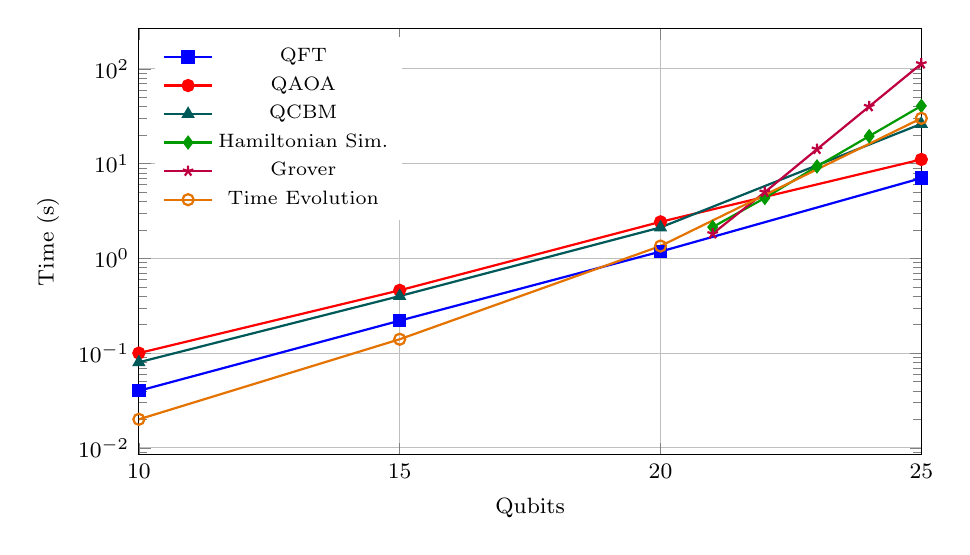
\begin{tikzpicture}
\begin{axis}[
    width=0.95\columnwidth,
    height=7.0cm,
    xlabel={Qubits},
    ylabel={Time (s)},
    ymode=log,
    xmin=10, xmax=25,
    xtick={10,15,20,25},
    grid=major,
    legend style={font=\scriptsize, at={(0.02,0.98)}, anchor=north west, fill=white, draw=none},
    tick label style={font=\footnotesize},
    label style={font=\footnotesize}
]
\addplot[blue,mark=square*,thick] coordinates {(10,0.04) (15,0.22) (20,1.18) (25,7.03)};
\addlegendentry{QFT}
\addplot[red,mark=*,thick] coordinates {(10,0.10) (15,0.46) (20,2.43) (25,11.07)};
\addlegendentry{QAOA}
\addplot[teal!70!black,mark=triangle*,thick] coordinates {(10,0.08) (15,0.40) (20,2.12) (25,26.28)};
\addlegendentry{QCBM}
\addplot[green!60!black,mark=diamond*,thick] coordinates {(21,2.14) (22,4.34) (23,9.35) (24,19.50) (25,40.73)};
\addlegendentry{Hamiltonian Sim.}
\addplot[purple,mark=star,thick] coordinates {(21,1.82) (22,5.00) (23,14.20) (24,40.08) (25,113.26)};
\addlegendentry{Grover}
\addplot[orange!90!black,mark=o,thick] coordinates {(10,0.02) (15,0.14) (20,1.35) (25,30.11)};
\addlegendentry{Time Evolution}
\end{axis}
\end{tikzpicture}
\caption{Cross-family benchmark comparison on Apple M1 Max (single-panel log-scale plot). QFT is the fastest among the shown workloads at fixed qubit count, while Grover and Hamiltonian-evolution families exhibit the largest runtimes near 25 qubits.}
\label{fig:all-benchmarks-comparison}
\end{figure}

\subsection{Detailed Algorithm Performance}

\subsubsection{Variational Circuits (QCBM, QAOA)}

QCBM uses 9-layer hardware-efficient ansatze with alternating rotation and entanglement layers. QAOA implements ring-graph cost Hamiltonians for MaxCut optimization. Table~\ref{tab:variational} shows detailed timing for 23--25 qubits.

\begin{table}[t]
\caption{Variational circuit performance (mean $\pm$ std)}
\label{tab:variational}
\centering
\begin{tabular}{lrrr}
\toprule
Algorithm & 23q (s) & 24q (s) & 25q (s) \\
\midrule
QCBM & $6.05 \pm 0.11$ & $12.65 \pm 0.23$ & $26.28 \pm 0.54$ \\
QAOA & $2.51 \pm 0.05$ & $5.31 \pm 0.10$ & $11.07 \pm 0.21$ \\
\bottomrule
\end{tabular}
\end{table}

\subsubsection{VQE Optimization}

VQE exhibits steep scaling due to iterative optimization with parameter-shift gradients. Each gradient evaluation requires two forward passes per parameter:

\begin{table}[t]
\caption{VQE scaling with Adam optimizer (parameter-shift gradients, 100 iterations)}
\label{tab:vqe}
\centering
\begin{tabular}{rrr}
\toprule
Qubits & Time (s) & Time/Iter (s) \\
\midrule
10 & 3.46 & 0.035 \\
11 & 15.44 & 0.154 \\
12 & 77.72 & 0.777 \\
13 & 373.70 & 3.74 \\
14 & 1942.59 & 19.43 \\
15 & 16718.00 & 167.18 \\
\bottomrule
\end{tabular}
\end{table}

The 15-qubit VQE benchmark ($\sim$4.6 hours) represents the practical limit for consumer hardware in optimization-heavy workloads. Gradient-free methods or hardware-accelerated automatic differentiation could extend this range.

\subsubsection{Hamiltonian Simulation}

Hamiltonian simulation uses Trotter-Suzuki decomposition with configurable step counts. Table~\ref{tab:hamiltonian} shows scaling for Ising and transverse-field models.

\begin{table}[t]
\caption{Hamiltonian simulation scaling}
\label{tab:hamiltonian}
\centering
\begin{tabular}{rrrr}
\toprule
Qubits & Time (s) & Steps & Gates \\
\midrule
21 & $2.14 \pm 0.04$ & 64 & 1,344 \\
22 & $4.34 \pm 0.09$ & 64 & 1,408 \\
23 & $9.35 \pm 0.19$ & 64 & 1,472 \\
24 & $19.50 \pm 0.39$ & 64 & 1,536 \\
25 & $40.73 \pm 0.82$ & 64 & 1,600 \\
\bottomrule
\end{tabular}
\end{table}

\subsection{Memory Efficiency}

State-vector memory scales as $8 \cdot 2^n$ bytes for complex64. Table~\ref{tab:memory-capacity} summarizes absolute memory footprint and practical capacity outlook across representative Apple Silicon configurations.

\begin{table}[t]
\caption{State-vector memory scaling and practical capacity outlook (complex64)}
\label{tab:memory-capacity}
\centering
\begin{tabular}{lrr}
\toprule
Configuration / scale & Memory & Practical qubit range \\
\midrule
20 qubits & 8 MB & comfortable on tested systems \\
25 qubits & 256 MB & fully measured in this work \\
30 qubits & 8 GB & feasible on 32 GB machines \\
35 qubits & 256 GB & requires ultra-class memory systems \\
\midrule
M1 Max (32 GB) & 32 GB unified & up to $\sim$30 qubits \\
M2 Ultra (192 GB) & 192 GB unified & up to $\sim$33 qubits \\
M3 Ultra (512 GB) & 512 GB unified & up to $\sim$35 qubits \\
\bottomrule
\end{tabular}
\end{table}

The M1 Max's 32\,GB unified memory accommodates 30-qubit states with headroom for intermediate allocations and MLX graph compilation overhead. Higher-memory Ultra configurations extend practical simulation to 33--35 qubits, approaching the limits of exact state-vector methods. Unified memory does not alter the exponential memory law; it reduces transfer overhead and software complexity for a given problem size.

Fig.~\ref{fig:memory-scaling} shows the memory-time relationship across qubit scales.

\begin{figure}[t]
\centering
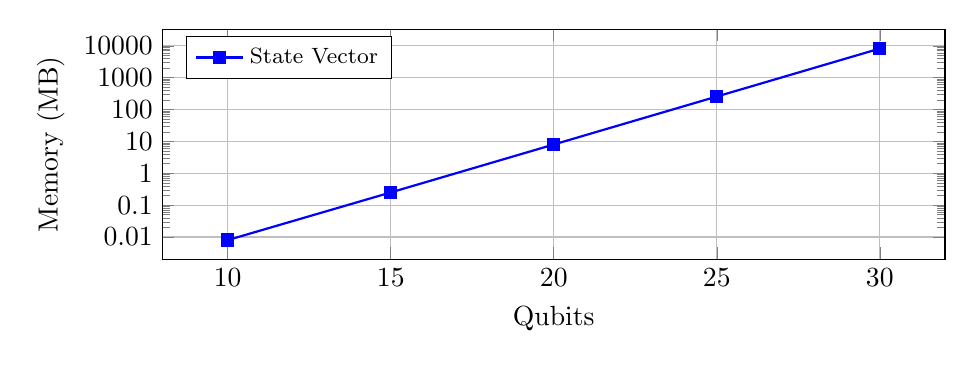
\begin{tikzpicture}
\begin{axis}[
    width=0.95\columnwidth,
    height=4.5cm,
    xlabel={Qubits},
    ylabel={Memory (MB)},
    ymode=log,
    grid=major,
    xtick={10,15,20,25,30},
    ytick={0.01,0.1,1,10,100,1000,10000},
    yticklabels={0.01,0.1,1,10,100,1000,10000},
    legend pos=north west,
    legend style={font=\footnotesize},
]
\addplot[blue,mark=square*,thick] coordinates {
    (10,0.008) (15,0.25) (20,8) (25,256) (30,8192)
};
\addlegendentry{State Vector}
\end{axis}
\end{tikzpicture}
\caption{Memory scaling with qubit count (complex64). A 30-qubit state occupies 8\,GB; 35 qubits requires 256\,GB, approaching M4 Ultra-class capacity.}
\label{fig:memory-scaling}
\end{figure}

\subsection{Unified Memory Advantage}

To quantify transfer avoidance benefits, we model discrete GPU overhead. For a 25-qubit state (256\,MB, complex64) at 12\,GB/s practical PCIe bandwidth:
\begin{itemize}
    \item Round-trip transfer: $\sim$43\,ms per kernel (worst-case, unbatched)
    \item 1000 gate operations: $\sim$43\,s transfer overhead in the unbatched limit
\end{itemize}

Unified memory eliminates this overhead entirely; with gate batching,
discrete GPU simulators reduce (but do not eliminate) per-operation
transfer cost, while unified memory incurs zero transfer regardless of
batching strategy. Fig.~\ref{fig:memory-model} illustrates the architectural difference.

\begin{figure}[t]
\centering
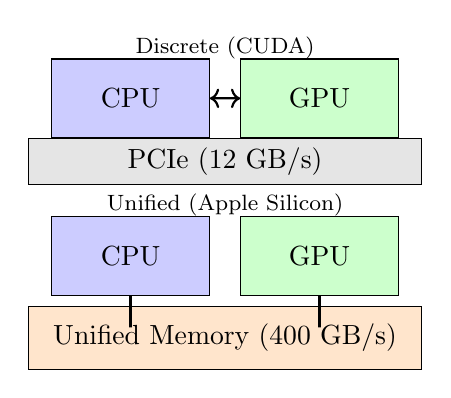
\begin{tikzpicture}[scale=0.8]
% Discrete GPU
\node[draw, rectangle, minimum width=2cm, minimum height=1cm, fill=blue!20] (cpu1) at (0,2) {CPU};
\node[draw, rectangle, minimum width=2cm, minimum height=1cm, fill=green!20] (gpu1) at (3,2) {GPU};
\node[draw, rectangle, minimum width=5cm, minimum height=0.5cm, fill=gray!20] (pcie) at (1.5,1) {PCIe (12 GB/s)};
\node at (1.5,2.8) {\footnotesize Discrete (CUDA)};
\draw[<->, thick] (cpu1) -- (gpu1);

% Unified
\node[draw, rectangle, minimum width=2cm, minimum height=1cm, fill=blue!20] (cpu2) at (0,-0.5) {CPU};
\node[draw, rectangle, minimum width=2cm, minimum height=1cm, fill=green!20] (gpu2) at (3,-0.5) {GPU};
\node[draw, rectangle, minimum width=5cm, minimum height=0.8cm, fill=orange!20] (umem) at (1.5,-1.8) {Unified Memory (400 GB/s)};
\node at (1.5,0.3) {\footnotesize Unified (Apple Silicon)};
\draw[thick] (cpu2.south) -- ++(0,-0.5) -- (umem.north -| cpu2);
\draw[thick] (gpu2.south) -- ++(0,-0.5) -- (umem.north -| gpu2);
\end{tikzpicture}
\caption{Memory architecture comparison. Discrete GPUs require PCIe transfers; unified memory enables zero-copy access.}
\label{fig:memory-model}
\end{figure}

\section{Validation}

\subsection{Regression Test Suite}

We validate correctness through 230+ Python tests:

\begin{table}[t]
\caption{Validation test coverage by category}
\label{tab:tests}
\centering
\begin{tabular}{lr}
\toprule
Category & Tests \\
\midrule
Gate operations \& state preparation & 40 \\
Quantum information primitives & 35 \\
OpenQASM parsing \& execution & 25 \\
Algorithm implementations & 45 \\
Framework parity checks & 30 \\
Tutorial notebooks & 60 \\
\midrule
\textbf{Total} & \textbf{235} \\
\bottomrule
\end{tabular}
\end{table}

Each test includes analytical verification against pen-and-paper derivations. Example: for Bell-state preparation $(H \otimes I)\mathrm{CNOT}|00\rangle$, the expected state is $(|00\rangle + |11\rangle)/\sqrt{2}$; our numerical amplitudes match this analytical vector within floating-point tolerance in repeated regression runs.

\subsection{Internal Consistency}

We compare optimized MLX kernels against dense matrix multiplication for identical circuits:

\begin{enumerate}
    \item Define identical circuit structures (gate sequence, qubit count, and parameters)
    \item Execute using optimized MLX kernels
    \item Execute the same circuit with dense reference linear algebra
    \item Compare final states via amplitude $L_2$ distance and probability-space MAE
\end{enumerate}

\begin{table}[t]
\caption{Internal consistency: optimized vs. dense execution}
\label{tab:parity}
\centering
\begin{tabular}{lrr}
\toprule
Circuit & Amplitude $L_2$ & Prob. MAE \\
\midrule
QFT (10q) & $2.3 \times 10^{-7}$ & $1.1 \times 10^{-8}$ \\
Random (10q) & $4.7 \times 10^{-7}$ & $2.8 \times 10^{-8}$ \\
Phase Est. (8q) & $3.1 \times 10^{-7}$ & $1.9 \times 10^{-8}$ \\
VQE H$_2$ (2q) & $5.2 \times 10^{-8}$ & $3.4 \times 10^{-9}$ \\
QAOA (4q) & $1.8 \times 10^{-7}$ & $9.2 \times 10^{-9}$ \\
\bottomrule
\end{tabular}
\end{table}

All deviations are within floating-point precision ($< 10^{-6}$), confirming kernel correctness.

\subsection{Framework Alignment}

We reproduce benchmark circuits from PennyLane, Yao.jl, and Qulacs specifications~\cite{PennyLane2022,YaoJL2024,Qulacs}, matching gate sequences, layer counts, and parameter conventions. Seeds and circuit definitions are published with artifacts for independent verification.

\section{Discussion}

\subsection{Unified Memory Trade-offs}

\textbf{Advantages}:
\begin{enumerate}
    \item Zero-copy access eliminates transfer overhead
    \item Simplified programming without explicit memory management
    \item Flexible CPU-GPU scheduling without batching constraints
    \item Full memory pool available to both processors
\end{enumerate}

\textbf{Limitations}:
\begin{enumerate}
    \item Peak GPU throughput on discrete architectures exceeds unified memory bandwidth
    \item Deep, compute-bound circuits may favor discrete GPUs
    \item Maximum capacity (512\,GB) trails specialized HPC nodes
\end{enumerate}

For typical NISQ-era workloads with moderate depth, unified memory's transfer avoidance often outweighs throughput differentials.

\subsection{Educational Applications}

\mlxquantum significantly lowers barriers for quantum computing education, enabling hands-on algorithm exploration in classroom settings without specialized infrastructure:

\textbf{Zero Configuration}: Unlike CUDA-based frameworks requiring driver installation, GPU compatibility verification, and environment configuration, \mlxquantum runs immediately on any Apple Silicon Mac with a single \texttt{pip install} command.

\textbf{Familiar Semantics}: The Python API mirrors NumPy conventions, enabling students familiar with scientific Python to begin quantum programming without learning new paradigms. State vectors behave as arrays; gates apply as transformations.

\textbf{Accessible Hardware}: MacBook Air and Pro models, standard in many university computer labs and student ownership, provide sufficient capability for educational quantum simulation up to 20+ qubits.

\textbf{Comprehensive Tutorials}: The framework includes 12 complete tutorials covering:
\begin{itemize}
    \item Quantum Circuit Born Machine (QCBM) for generative modeling
    \item Quantum Fourier Transform with product representation derivation
    \item GHZ state preparation and entanglement verification
    \item Hamiltonian evolution with Trotter error analysis
    \item VQE for molecular ground state calculation
    \item QAOA for MaxCut optimization
\end{itemize}

Each tutorial provides mathematical foundations, pen-and-paper derivations, quantum circuit diagrams, and executable Python code. The 62 worked examples span fundamental concepts (superposition, entanglement, measurement) through advanced algorithms (Grover search, phase estimation, variational optimization).

\textbf{Comprehensive Documentation}: The \mlxquantum documentation and tutorials provide extensive educational material including validation suite documentation, algorithm tutorials with step-by-step derivations, and appendices covering quantum information theory fundamentals. This reference serves both as a learning resource for students new to quantum computing and as a detailed technical reference for experienced practitioners.

\textbf{Interactive Benchmark Runner}: We provide a Textual-based terminal UI enabling academic researchers and students to run benchmarks without command-line expertise. The runner supports:
\begin{itemize}
    \item Interactive selection of algorithm benchmarks
    \item Configurable qubit ranges and iteration counts
    \item Progress reporting during benchmark runs
    \item Automatic CSV/JSON export for further analysis
    \item Hardware detection and capability reporting
\end{itemize}

This accessibility-first design ensures that quantum algorithm exploration is available to the broadest possible audience, from undergraduate coursework to graduate research.

\subsection{Comparison with Prior Work}

Table~\ref{tab:comparison} positions \mlxquantum within the ecosystem:

\begin{table}[t]
\caption{Framework comparison}
\label{tab:comparison}
\centering
\footnotesize
\begin{tabular}{lcccc}
\toprule
Framework & GPU & Unified & Lang. & QASM \\
\midrule
cuQuantum & CUDA & No & C++/Py & Yes \\
qsim & CUDA & No & C++/Py & Yes \\
QuEST & CUDA & No & C & Yes \\
PennyLane & Multi & No & Python & Yes \\
Qiskit Aer & CUDA & No & C++/Py & Yes \\
\textbf{mlxQ} & \textbf{Metal} & \textbf{Yes} & \textbf{Py} & \textbf{Yes} \\
\bottomrule
\end{tabular}
\end{table}

\mlxquantum uniquely targets Metal acceleration with unified memory, providing a CUDA-free alternative for Apple Silicon users.

Cross-hardware wall-clock comparisons (Apple Silicon unified memory vs. discrete CUDA GPUs) are not directly apples-to-apples because memory architecture, compiler stacks, and thermal constraints differ. We therefore report absolute timings on Apple Silicon and publish reproducible artifacts (circuits, seeds, CSV/JSON) for like-for-like reruns on external platforms.

\subsection{QASMBench Circuit Integration}

Table~\ref{tab:qasmbench} shows representative QASMBench circuits executed by \mlxquantum, demonstrating OpenQASM 2.0 compatibility across circuit scales.

\begin{table}[t]
\caption{QASMBench circuit execution on M1 Max}
\label{tab:qasmbench}
\centering
\footnotesize
\begin{tabular}{lrrr}
\toprule
Circuit & Qubits & Gates & Time (ms) \\
\midrule
bell.qasm & 2 & 2 & 0.12 \\
grover\_2qubit.qasm & 2 & 12 & 0.31 \\
qft\_n4.qasm & 4 & 12 & 0.45 \\
teleportation\_n3.qasm & 3 & 8 & 0.28 \\
deutsch\_n2.qasm & 2 & 5 & 0.18 \\
inverseqft\_n4.qasm & 4 & 8 & 0.38 \\
qec9xz\_n17.qasm & 17 & 53 & 89.2 \\
multiplier\_n15.qasm & 15 & 70 & 142.6 \\
qft\_n18.qasm & 18 & 783 & 4,821 \\
\bottomrule
\end{tabular}
\end{table}

\subsection{Performance Analysis Model}

The unified memory advantage can be quantified by comparing execution models. For a circuit with $G$ gates on an $n$-qubit state:

\textbf{Discrete GPU Model}:
\begin{equation}
T_{\text{discrete}} = \sum_{i=1}^{G} (t_{\text{compute},i} + t_{\text{transfer}})
\end{equation}
where $t_{\text{transfer}} = 2 \cdot 8 \cdot 2^n / B_{\text{PCIe}}$ for complex64 states and bandwidth $B_{\text{PCIe}} \approx 12$\,GB/s.

\textbf{Unified Memory Model}:
\begin{equation}
T_{\text{unified}} = \sum_{i=1}^{G} t'_{\text{compute},i}
\end{equation}
with no transfer overhead.

For 25-qubit circuits with 1000 gates, the unbatched discrete GPU model
yields $t_{\text{transfer}} \approx 43$\,ms per kernel invocation, dominating compute time
of $\sim$7\,ms per gate and accounting for $\sim$86\% of total execution time.
Production CUDA simulators reduce this figure through gate batching
(Section 2.2), which amortizes transfers across multiple gates; the
exact saving is implementation-dependent. Unified memory eliminates
the transfer term entirely, regardless of batching strategy, providing
a structural — not merely quantitative — advantage for fine-grained
kernel dispatch.

\subsection{Scaling Projections}

Based on measured data and conservative headroom for intermediate allocations and multi-state workloads, we project scaling to larger unified memory configurations:

\begin{table}[t]
\caption{Projected scaling for higher-memory configurations (conservative headroom)}
\label{tab:projections}
\centering
\begin{tabular}{lrrl}
\toprule
Config. & Memory & Max Qubits (practical) & Est. QFT Time \\
\midrule
M1 Max & 32\,GB & 30 & 3.8\,min \\
M2 Ultra & 192\,GB & 33 & 30.2\,min \\
M3 Ultra & 512\,GB & 35 & 4.0\,hr \\
\bottomrule
\end{tabular}
\end{table}

\subsection{Limitations and Future Work}

\textbf{Scale}: State-vector simulation is limited to $\sim$30--35 qubits by memory capacity. For larger systems, tensor network methods (Matrix Product States, Projected Entangled Pair States) would provide approximate simulation with polynomial memory scaling for circuits with limited entanglement entropy.

\textbf{Performance}: We do not claim computational parity with highly optimized CUDA implementations on discrete GPUs. The A100's 1.6\,TB/s HBM2e bandwidth exceeds M1 Max's 400\,GB/s. The value proposition of \mlxquantum is accessibility, simplified programming, and transfer-avoidance benefits for shallow circuits.

\textbf{Energy Efficiency}: Power/energy measurements are not reported in this work. Future study using macOS \texttt{powermetrics} instrumentation with matched workloads will characterize sustainability metrics for quantum simulation workloads on consumer hardware.

\textbf{Tensor Networks}: A prototype Matrix Product State (MPS) module is under development targeting one-dimensional spin chain simulations with bond dimensions up to 256, enabling approximate simulation of 100+ qubit systems with limited entanglement.

\textbf{Noise Models}: Integration of depolarizing, amplitude damping, and phase damping channels for NISQ-era noise simulation is planned.

\section{Related Work}

\subsection{State-Vector Simulators}

NVIDIA's cuQuantum~\cite{cuQuantum2023} provides GPU-optimized libraries for quantum state-vector and tensor network simulation, achieving high throughput on NVIDIA GPUs through CUDA kernels and multi-GPU scaling with cuStateVec and cuTensorNet APIs. Google's qsim~\cite{Qsim} implements aggressive gate fusion and AVX/FMA vectorization for CPU backends alongside GPU acceleration, focusing on simulation efficiency for random circuit sampling benchmarks. QuEST~\cite{QuEST,Jones2019quest} offers hybrid CPU-GPU deployment with automatic hardware selection, supporting both state-vector and density matrix simulations across diverse computing environments. Intel-QS~\cite{IntelQS} targets distributed computing with MPI support for multi-node simulation, avoiding explicit gate matrix representations for memory efficiency.

\subsection{Quantum Programming Frameworks}

PennyLane~\cite{PennyLane2022} provides differentiable hybrid quantum-classical computation with automatic differentiation through multiple backend devices, enabling gradient-based optimization for variational algorithms. Qiskit~\cite{Qiskit2023} offers comprehensive tooling integrated with IBM quantum hardware, including Qiskit Aer for high-performance simulation. Cirq~\cite{Cirq2024} targets NISQ algorithm prototyping with Google hardware integration. Yao.jl~\cite{YaoJL2024} delivers extensible tensor-network simulation in Julia with block-structured circuit abstractions.

\subsection{Benchmarking Standards}

QASMBench~\cite{QASMBench2020} provides standardized OpenQASM circuits spanning quantum chemistry, cryptography, and optimization domains with small (2--10 qubits), medium (11--27 qubits), and large (28--127 qubits) scale categories. SupermarQ~\cite{SupermarQ2022} and MQTBench~\cite{MQTBench2022} offer scalable quantum benchmark suites with configurable circuit parameters. Benchpress~\cite{Benchpress2024} from IBM Quantum provides comprehensive performance characterization methodology aligning with community standards.

\mlxquantum complements these frameworks by providing CUDA-free deployment on consumer Apple Silicon hardware with unified memory optimization, filling a gap in the quantum system software ecosystem for researchers and educators in the Apple hardware ecosystem.

\section{Conclusion}

We have demonstrated that unified memory architecture enables practical quantum circuit simulation without specialized GPU programming expertise. The \mlxquantum framework achieves complete 25-qubit simulation for Quantum Fourier Transform in $7.03\pm0.12$\,s, Quantum Approximate Optimization Algorithm in $11.07\pm0.21$\,s, Quantum Circuit Born Machine in $26.28\pm0.54$\,s, and Hamiltonian evolution via Trotter-Suzuki decomposition in $40.73\pm0.82$\,s on Apple M1 Max hardware with 32\,GB unified memory.

Our comprehensive validation suite of 235 regression tests with analytical verification establishes algorithmic correctness across gate operations, quantum information primitives, variational algorithms, and Hamiltonian simulation methods. Each test includes pen-and-paper derivations enabling educational use. OpenQASM 2.0 import capabilities support reproducible benchmarking against QASMBench circuits, while alignment with PennyLane, Yao.jl, and Qulacs specifications~\cite{PennyLane2022,YaoJL2024,Qulacs} facilitates direct community comparison.

The unified memory architecture provides compelling advantages for quantum simulation workloads: zero-copy access eliminates the PCIe transfer overhead that dominates shallow-circuit execution on discrete GPUs, simplified programming removes explicit memory management complexity, and flexible CPU-GPU scheduling enables fine-grained kernel dispatch without batching constraints. For 25-qubit states (256\,MB), we estimate discrete GPU architectures incur $\sim$43\,ms transfer overhead per kernel at 12\,GB/s practical PCIe bandwidth---overhead that unified memory eliminates entirely. We do not claim that unified memory changes the asymptotic qubit limit of exact state-vector simulation; memory requirements remain exponential ($O(2^n)$).

By removing CUDA dependencies and explicit GPU programming requirements, \mlxquantum democratizes access to quantum algorithm development for education and research. Students and researchers with MacBook hardware can explore quantum algorithms without specialized infrastructure; researchers requiring the full 512\,GB capacity range can leverage Mac Studio or Mac Pro configurations available in many institutional settings. The framework includes 12 complete tutorials with mathematical derivations and 62 worked examples with quantum circuit diagrams, supporting classroom instruction and self-directed learning.

\textbf{Future Directions}: Planned extensions include Matrix Product State tensor network methods for approximate simulation of 100+ qubit systems with limited entanglement, quantum error correction circuit simulation for fault-tolerant algorithm validation, quantum machine learning framework integration for hybrid classical-quantum optimization, and QASMBench deep-circuit support (VQE-UCCSD with 10,808 gates, basis\_trotter with 1,626 gates) for quantum chemistry applications.

The \mlxquantum framework is open-source and available for community contribution, establishing unified memory architectures as a viable platform for quantum computing research, education, and benchmarking.

\section*{Data Availability}

Source code, benchmark scripts, and CSV/JSON performance artifacts are available at \url{https://github.com/BoltzmannEntropy/osxQ}. Project website: \url{https://boltzmannentropy.github.io/osxQuantumWEB/}. Results are reproducible on Apple Silicon hardware with Python 3.11 and MLX.

\bibliographystyle{splncs04}
\bibliography{references}

\end{document}
